\section{Experimental validation}\label{sec:experiments}

% Please add the following required packages to your document preamble:
% \usepackage{booktabs}
% \usepackage{graphicx}
\begin{table}[]
    \centering
    \caption{Hardware used in the experiments.}\label{tab:hardware}
    \resizebox{\columnwidth}{!}{%
    \begin{tabular}{@{}llrrrl@{}}
    \toprule
    \multicolumn{1}{c}{\textbf{}} &
      \multicolumn{1}{c}{\textbf{CPU}} &
      \multicolumn{1}{c}{\textbf{\begin{tabular}[c]{@{}c@{}}Freq\\ {[}\si{\giga\hertz}{]}\end{tabular}}} &
      \multicolumn{1}{c}{\textbf{\begin{tabular}[c]{@{}c@{}}Core\\ Count\end{tabular}}} &
      \multicolumn{1}{c}{\textbf{\begin{tabular}[c]{@{}c@{}}RAM\\ {[}\si{\giga\byte}{]}\end{tabular}}} &
      \multicolumn{1}{c}{\textbf{\begin{tabular}[c]{@{}c@{}}Operating\\ System\end{tabular}}} \\ \midrule
    \textbf{Cloudlet} &
      \begin{tabular}[c]{@{}l@{}}Intel\textregistered{} Core\texttrademark{}\\ i7-8700\end{tabular} &
      \num{3.2} &
      \num{6} &
      \num{32} &
      \begin{tabular}[c]{@{}l@{}}Ubuntu Server \\20.04 LTS \\Kernel v5.4.0\\\ \end{tabular} \\
    \textbf{Client} &
      \begin{tabular}[c]{@{}l@{}}Cortex-A72\\ (ARM v8)\end{tabular} &
      \num{2.0} &
      \num{4} &
      \num{8} &
      \begin{tabular}[c]{@{}l@{}}Ubuntu Server \\20.04 LTS \\Kernel v5.4.0\end{tabular} \\ \bottomrule
    \end{tabular}%
    }
\end{table}

In this section, we demonstrate the practical utility of \ac{CLEAVE} through a series of experiments on an emulated \ac{NCS} running between a client device and a cloudlet.
We aim to answer question relating to the ability of our framework to provide relevant, accurate, and repeatable measurements of the performance of \acp{NCS} deployed on edge computing infrastructure.

This section is structured in two parts.
\Cref{ssec:expsetup} details the experimental setup and describes the experiments performed.
\Cref{ssec:results} then presents and discusses the numerical results.

\subsection{Experimental Setup}\label{ssec:expsetup}

The \acl{NCS} employed for these experiments corresponds to an inverted pendulum, chosen for to its relative simplicity as well as prevalence in the field of automatic control as one of the fundamental examples of linear control.
The physical system, represented in \cref{fig:invpend}, is implemented as a real-time discrete-time physical emulation using CLEAVE's API and a 2D physics library~\autocite{chipmunk2d,pymunk}, executed at a constant \SI{120}{\hertz}.
For the controller, a proportional-differential strategy is employed, implemented using the framework Controller API and the NumPy numeric computation library~\autocite{harris2020array}.

\begin{figure}
    \centering
    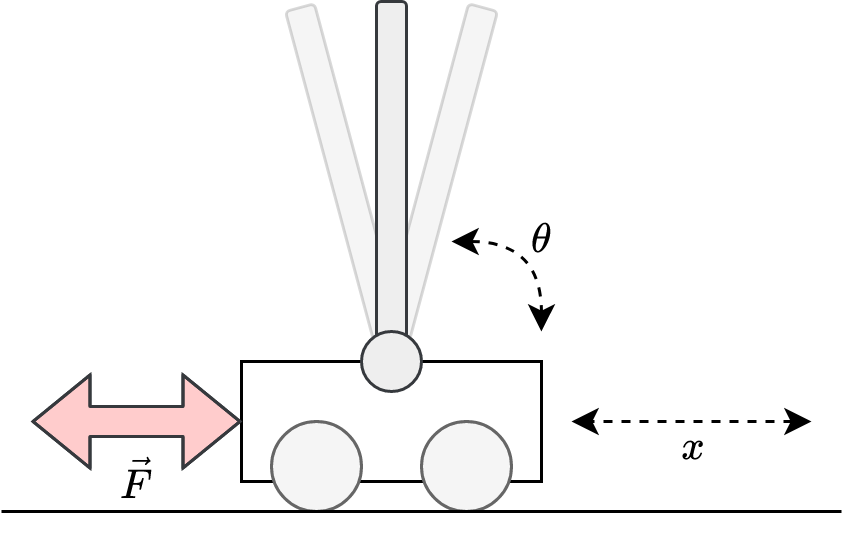
\includegraphics[width=.95\columnwidth]{images/inverted_pendulum.png}
    \caption{
        The two-dimensional inverted pendulum system.
        The cart moves on the X-axis, and the pendulum on top of it swings freely.
        The objective of the system is to balance the pendulum vertically through the application of horizontal forces on the cart.
    }\label{fig:invpend}
\end{figure}

We depict our experimental edge setup in \cref{fig:cleave:expsetup}, consisting of a single control loop deployed across a pair of consumer-grade computing devices.
We employ a Raspberry Pi 4B single-board computer as a client device, together with a general-purpose \verb|x86_64|-based workstation which acts as the cloudlet.
These devices are connected to each other by an 802.11n WiFi link.
For ease of orchestration and re-parametrization, as well as to mimic real-world deployments, we package our CLEAVE control loop as a pair of Docker~\cite{merkel2014docker} containers.
For our main set of experiments, a two-node Docker \emph{Swarm}~\cite{Swarm2021} is set up with the cloudlet host configured as a Manager and the client device as a Worker node.
The containers are deployed inside the Swarm, with one of them configured as a Controller, assigned to the cloudlet, and the other one as the Inverted Pendulum Plant and assigned to the client.
These instances communicate using the \ac{UDP} over an overlay network which sits on top of and abstracts away the real network configuration.
Additionally, to obtain baseline results without the stochastic effects of the network, we employ a secondary ``local-only'' setup, in which we simply execute both Plant and Controller containers co-located on the cloudlet.

\begin{figure}
    \centering
    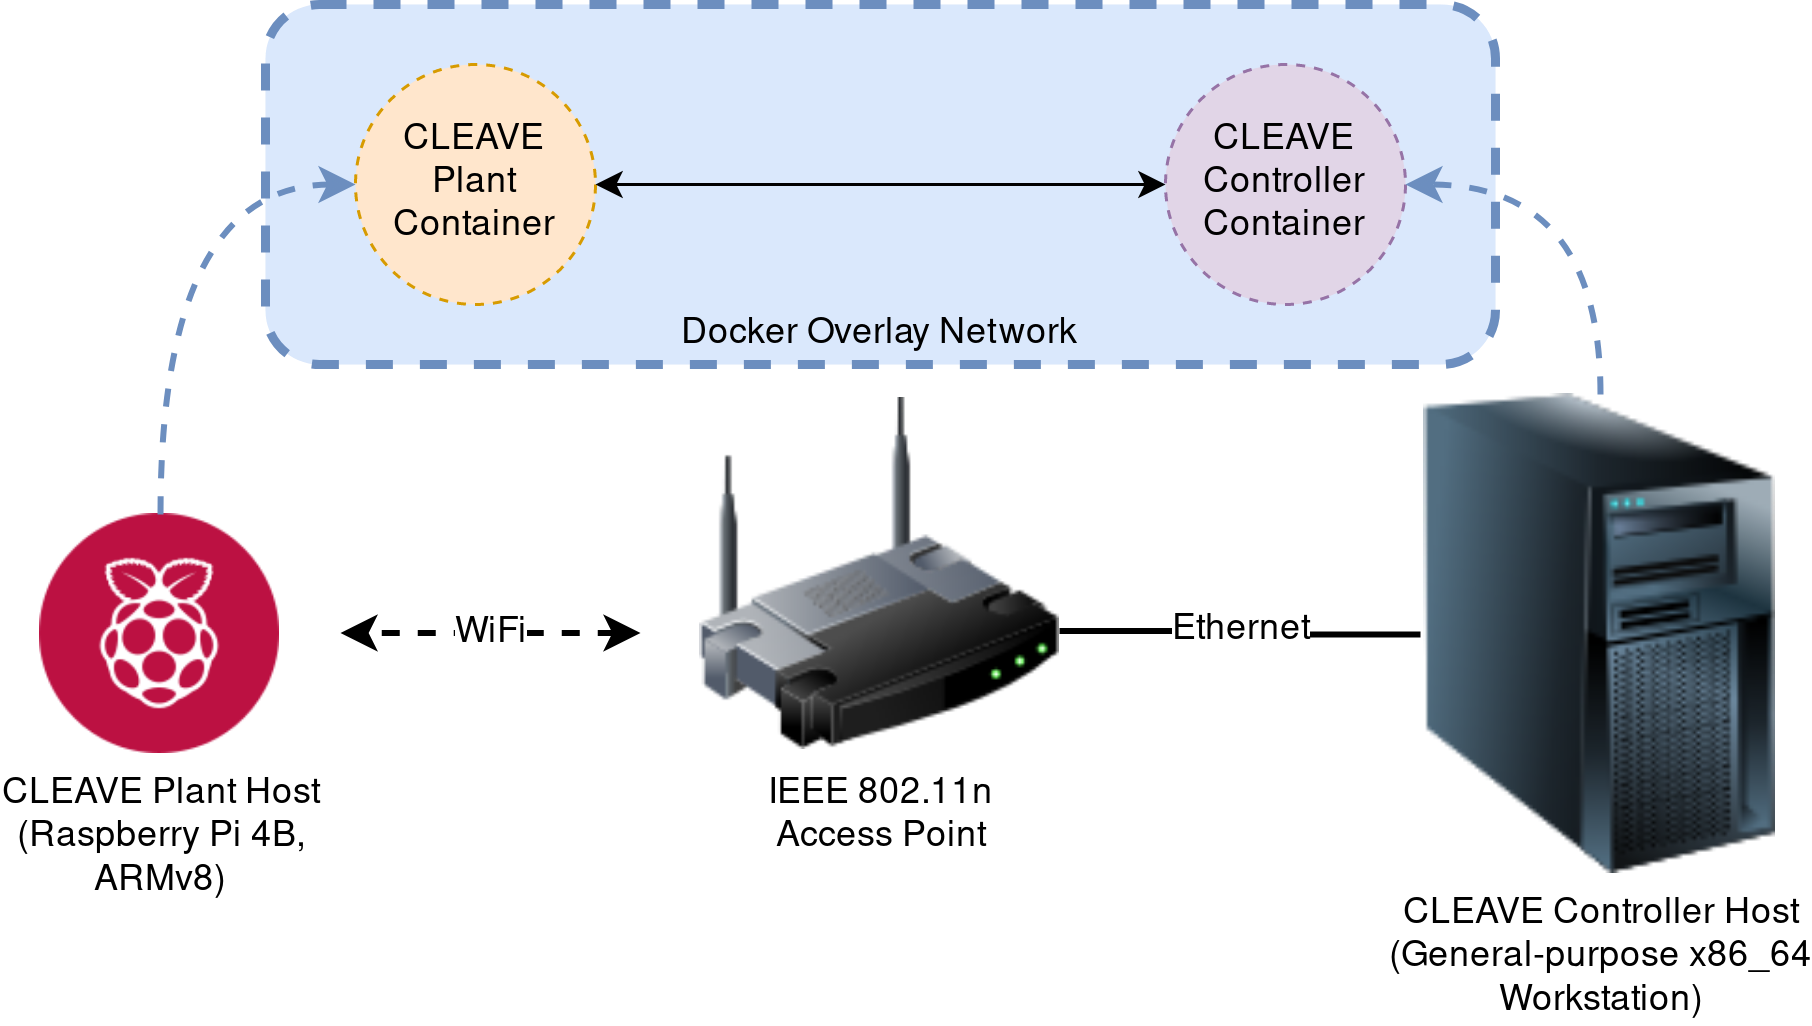
\includegraphics[width=.95\columnwidth]{images/CLEAVE_experiment_setup}
    \caption{Experimental setup. Containerized versions of the core CLEAVE emulation components are deployed inside a Docker Swarm Overlay Network spanning a Raspberry Pi 4B Plant host connected to an x86 Controller host over a 802.11n WiFi link.}\label{fig:cleave:expsetup}
\end{figure}

These setups are then used to run a series of experiments with varying parametrization of the controlled system.
Specifically, we modify:
\begin{itemize}
    \item the sampling rate of the Plant state, setting it to \SIlist[list-units=single,list-final-separator={, or }]{5;10;20;40;60}{\hertz};
    \item the responsiveness of the Controller, by adding fixed delays of  \SIlist[list-units=single,list-final-separator={, or }]{0;25;50;100}{\milli\second} after the processing of each sample.
\end{itemize}
We repeat each combination of these parameters at least \num{10} times, for both the networked and ``local-only'' setups; experiments with interesting and relevant results are then repeated an additional \num{20} times for better statistical significance in the results.
During each repetition, we collect detailed data on both the state of the controlled system as well as on the data sent over the network.

\subsection{Results}\label{ssec:results}

The results presented below provide valuable insights on both system limits and on the chosen \ac{NCS} itself, as well as on the capabilities of \ac{CLEAVE}.

We begin with a simple analysis of the stability of the Plant.
\Cref{fig:topple:fraction} shows a visualization of the fraction of plants that toppled in each scenario.
It provides a very clear overview of the minimum requirements 

\begin{figure}
    \centering
    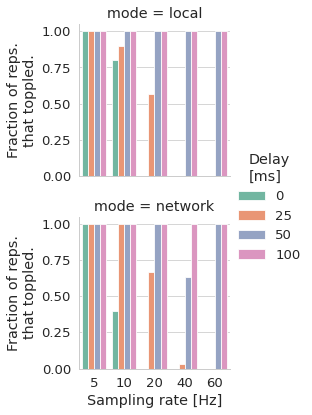
\includegraphics[width=.8\columnwidth]{topple_fraction.png}
    \caption{Fraction of plants that toppled, per experimental setup.}%
    \label{fig:topple:fraction}
\end{figure}

When it comes to network reliability, mean packet losses for all setups were below \SI{0.15}{\percent}. 
\todo[inline]{Discuss which network results to add.}